\section{Event-Aligned Spline Actions}
\label{sec:method}

Let $o_t$ denote images, $s_t$ robot state, and $\ell_t$ the active instruction. A conventional chunking VLA predicts $H$ future actions from $(o_t,s_t,\ell_t)$. We retain its vision--language backbone and flow-matching action expert, but change the prediction targets and decoder (Fig.~\ref{fig:method}).

\begin{figure*}[t]
\centering
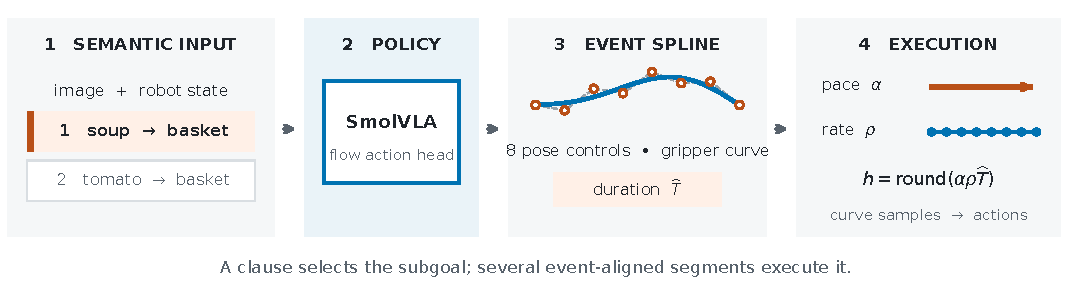
\includegraphics[width=\textwidth]{figures/method_v4.pdf}
\caption{The active clause conditions an unchanged VLA backbone. Each query produces a short spline segment and its duration. The decoder chooses the number of issued actions using duration scale $\alpha$ and control-rate ratio $\rho$. Clause switching occurs on a separate, slower schedule; it is held identical across heads in the primary language comparison.}
\label{fig:method}
\end{figure*}

\subsection{A Short Motion Program}

For a window of $T$ pose-delta commands $a^{\mathrm{pose}}_0,\ldots,a^{\mathrm{pose}}_{T-1}$, form the cumulative command path
\begin{equation}
 p_0=0,\qquad p_k=\sum_{j=0}^{k-1}a^{\mathrm{pose}}_j.
\end{equation}
This path is expressed in the controller's command coordinates. It is not a reconstruction of the measured end-effector pose, and summing rotational command components is not an exact composition on $SO(3)$. We approximate it with a clamped, uniform cubic B-spline,
\begin{equation}
 p(u)=\sum_{i=0}^{n-1} B_{i,3}(u)c_i,\qquad u\in[0,1],\quad n=8.
 \label{eq:curve}
\end{equation}
The training fit pins $c_0=0$ and $c_{n-1}=p_T$. The remaining controls minimize
\begin{equation}
 \sum_{k=0}^{T}\left\|p(k/T)-p_k\right\|_2^2.
 \label{eq:fit}
\end{equation}
We precompute the least-squares operators for each allowed duration. The gripper command is fitted directly, without cumulative summation, and thresholded by sign during decoding. In RoboCasa's mobile-manipulator action layout, base and mode commands occupy additional fitted channels rather than pose-delta channels.

Each output token contains one pose control point, one gripper control value, and a replicated duration target $\log T$. The action expert therefore emits eight tokens rather than the waypoint head's 50. We standardize targets per token and train with the same conditional flow-matching objective \cite{shukor2025smolvla,lipman2023flow}. At inference, we average the predicted log durations, $\bar z=\frac1n\sum_i\widehat{\log T}_i$, and decode
\begin{equation}
 \widehat T=\operatorname{clip}\!\left(
 \operatorname{round}(e^{\bar z}),T_{\min},T_{\max}\right).
 \label{eq:duration}
\end{equation}
We reset the predicted starting control point to zero. The predicted endpoint remains learned; endpoint-preserving resampling preserves that prediction, not necessarily the demonstrated endpoint or the robot's realized path.

\subsection{Event-Aligned Supervision}

Starting at each training frame, we select the first boundary after $T_{\min}=8$ commands. A boundary is a gripper-command transition, two consecutive pose-command norms below 0.15 times the window median, or episode padding. If none occurs, the window ends at $T_{\max}=24$ commands (16 for CALVIN). A boundary at index $k$ gives $T=k$: commands $0,\ldots,k-1$ enter the fit, while the boundary command belongs to the next segment. Thus duration predicts an action event or cap, not a semantic subgoal label.

This distinction matters for language supervision. Gripper and pause events provide short motion boundaries, but a task clause may require several grasps, transports, or contact corrections. Event-aligned targets do not impose a one-to-one correspondence between language clauses and spline segments.

\subsection{Executable Clauses}

A program is an ordered list $\mathcal L=(\ell^1,\ldots,\ell^M)$. At any time, the active clause replaces the whole-task caption in the policy input. A scheduler advances the clause pointer and clears queued actions generated under the previous instruction. There is no additional high-level model.

For the two-subgoal LIBERO study, we label each demonstration with two clauses. The split is the first gripper release following at least 48 consecutive closed commands; the release is assigned to the first clause, and the next observation--action pair begins the second. The two training views have identical images, states, actions, and episode membership. Only language metadata changes.

The main comparison uses an outcome-independent, fixed clause clock for both heads. The switch occurs at the median labeled transition in the training demonstrations: step 139 for the soup/tomato task and 107 for the two-mug task. A second condition switches at an executed close-to-open gripper command. The order diagnostic instead uses the official subgoal predicate to advance the clause; this privileged scheduler isolates the order request from completion-detection errors and is not a deployable result.

\subsection{Controlling the Physical Clock}

Let $f_0$ be the action rate used to interpret the training commands, $f$ the execution rate, and $\rho=f/f_0$. A duration multiplier $\alpha$ yields
\begin{equation}
 \begin{aligned}
 h&=\max\{2,\operatorname{round}(\alpha\rho\widehat T)\},\\
 a_j^{\mathrm{pose}}&=p((j+1)/h)-p(j/h).
 \end{aligned}
 \label{eq:decode}
\end{equation}
Ignoring rounding and actuator clipping, execution time is $h/f\approx\alpha\widehat T/f_0$. Changing $\alpha$ therefore changes pace; changing $\rho$ at fixed $\alpha$ changes sampling density while preserving duration. The underlying predicted curve is unchanged. The gripper curve is sampled on the corresponding grid and sign-thresholded. As with the original controller, issued pose commands are bounded.

This factorization guarantees a shared predicted endpoint across sampling grids before clipping. It does not guarantee unchanged closed-loop outcomes, tracking at arbitrary speeds, or derivative continuity across replans. We use ordinary receding-horizon execution: issue up to $K$ actions from a segment, observe the robot again, and replan. A segment shorter than $K$ drains the queue earlier.

\textbf{Waypoint interpolation baseline.} The same timing operation can be applied to a waypoint prediction. Denormalize its per-step deltas, accumulate them into a path $q_k$, linearly interpolate that path at $h+1$ equally spaced phases, and difference successive samples. The gripper uses nearest-step sampling and sign thresholding. Finally, renormalize if the policy's saved postprocessor expects normalized actions. Interpolating normalized deltas directly is incorrect: adding a per-step mean after changing the number of commands changes the total displacement. This baseline needs no retraining and is distinct from repeating unchanged waypoints at another rate.
